\section{Theory}
\subsection{Derivation of Cauchy equation}
This week we are dealing with the Cauchy equation, also known as the motion equation. We will define it in terms of material coordinates which gives us $\rho_0 \ddot{\mathbf{x}} = \mathbf{b}_0 + \nabla_{\mathbf{X}}\cdot \mathbf{P}$ where $\rho_0$ is the mass density in material coordinates, $\ddot{\mathbf{x}}$ is the spatial acceleration, $\mathbf{b}_0$ is the body force densities and $\nabla_{\mathbf{X}}\cdot \mathbf{P}$ is the divergence with respect to the material coordinates of the stress tensor. We can now apply the Finite Volume Method to our partial differential equation. The first step is to take the volume integral over our equation. We let $A_i$ denote the control volume of the \textit{i'th} vertex and get:
\begin{equation*}
	\int_{A_i}\rho_0 \ddot{\mathbf{x}}_i dA = \int_{A_i}\mathbf{b}_0dA + \int_{A_i}\nabla_{\mathbf{X}}\cdot \mathbf{P}dA
\end{equation*}
We would now like to simplify the term $\int_{A_i}\rho_0 \ddot{\mathbf{x}}_i dA$ by applying a midpoint approximation, but because $\ddot{\mathbf{x}}_i$ depends on time we first need to apply Leibniz' rule to move the time derivative outside the integral. We can then apply the midpoint approximation by simply removing the integral and multiplying with $A_i$. As we now have both the area and density we can combine these terms into a single term of mass, $m_i$. As the mass does not depend on time we are left with:
\begin{equation*}
	m_i\ddot{\mathbf{x}}_i = \int_{A_i}\mathbf{b}_0dA + \int_{A_i}\nabla_{\mathbf{X}}\cdot \mathbf{P}dA
\end{equation*}
For the term $\int_{A_i}\mathbf{b}_0dA$ we can directly apply the midpoint approximation and get:
\begin{equation*}
	m_i\ddot{\mathbf{x}}_i = \mathbf{b}_0A_i + \int_{A_i}\nabla_{\mathbf{X}}\cdot \mathbf{P}dA
\end{equation*}
For the last term $\int_{A_i}\nabla_{\mathbf{X}}\cdot \mathbf{P}dA$ we apply Gauss-divergence theorem to convert the volume integral to a surface integral:
\begin{equation*}
	m_i\ddot{\mathbf{x}}_i = \mathbf{b}_0A_i + \int_{S}\mathbf{P}\mathbf{N}dS
\end{equation*}
We can now exploit that our surfaces are piecewise continuous and integrate over each edge piece:
\begin{equation*}
	m_i\ddot{\mathbf{x}}_i = \mathbf{b}_0A_i + \sum_e \sum_{\gamma\in \{\alpha,\beta\}} \int_{S^e_\gamma}\mathbf{P}\mathbf{N}dS
\end{equation*}
Where \textit{e} denotes our edges in the control volumes. Due to the choice of using median dual vertex centered control volumes, we can split the control volume edges into two, $\alpha$ and $\beta$. This is illustrated in \autoref{controlvolume}.

\begin{figure}
	\centering
	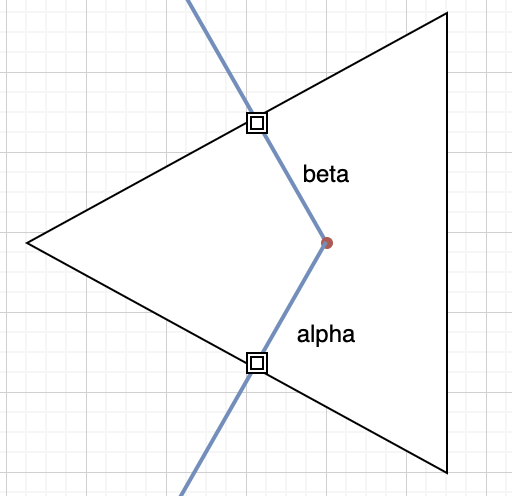
\includegraphics[width=0.4\linewidth]{Materials/controlvolume}
	\caption{A single triangle in the mesh (in black) with the control volume (in blue) going through it. We note the control volume goes from the midpoints on the triangle mesh to the center of triangles. Because of this we can split the control volume surface in two pieces, $\alpha$ and $\beta$.}
	\label{controlvolume}
\end{figure}

We can now apply boundary conditions. Here we split the term $\int_{S^e_\gamma}\mathbf{P}\mathbf{N}dS$ into three boundaries terms. The first one being the free boundaries where no traction is applied, and is given by $\mathbf{t} = \mathbf{P}\mathbf{N} = 0$ and thus giving us:
\begin{equation*}
	\int_{S^e_\gamma}\mathbf{P}\mathbf{N}dS = 0
\end{equation*}
The second type being the non-free boundaries, where we apply some known amount of traction giving us:
\begin{equation*}
	\int_{S^e_\gamma}\mathbf{P}\mathbf{N}dS = \mathbf{t}l^e_\gamma
\end{equation*}
where $l^e_\gamma$ is the length of the boundary piece. And the last one being the internal boundaries which we 'pull out'. We thus split the summation into two (the term for the free boundaries simply disappear):
\begin{equation*}
	m_i\ddot{\mathbf{x}}_i = \mathbf{b}_0A_i + \sum_{e_{traction}}  \mathbf{t}l^{e_{traction}}_\gamma + \sum_{e_{inner}} \sum_{\gamma\in \{\alpha,\beta\}} \int_{S^{e_{inner}}_\gamma}\mathbf{P}\mathbf{N}dS
\end{equation*} 
To simplify a little, we can define $\mathbf{f}^{ext}_i =  \mathbf{b}_0A_i$ as this models the external forces and $\mathbf{f}^t_i = \sum_{e_{traction}}  \mathbf{t}l^{e_{traction}}_\gamma$ as this models the traction forces. We then have:
\begin{equation*}
	m_i\ddot{\mathbf{x}}_i = \mathbf{f}^{ext}_i + \mathbf{f}^t_i + \sum_{e_{inner}} \sum_{\gamma\in \{\alpha,\beta\}} \int_{S^{e_{inner}}_\gamma}\mathbf{P}\mathbf{N}dS
\end{equation*}

We can now look at the deformation gradient. To go from spatial coordinates to material coordinates we have the relation $\mathbf{x} = \phi(\mathbf{X})$. The deformation gradient is the derivative of the spatial coordinates with respect to the material coordinates, and is thus defined as:
\begin{equation*}
	\mathbf{F} = \frac{\partial \mathbf{x}}{\partial \mathbf{X}} = \frac{\partial \phi}{\partial \mathbf{X}}
\end{equation*}
We can also think of the deformation gradient as a differentiable, and we then have:
\begin{equation*}
	d\mathbf{x} = \mathbf{F}d\mathbf{X}
\end{equation*}
If we assume the coordinates changes linearly over our triangles, that means the deformation gradient will be constant for all vectors on the triangles. To compute the deformation gradient we can thus take two points on our triangle in spatial coordinates, $a$ and $b$, and their corresponding location in material coordinates, $A$ and $B$, and then we have the following relations:
\begin{align*}
	a &= \mathbf{F}A\\
	b &= \mathbf{F}B
\end{align*} 
This can be combined and written as a linear system:
\begin{equation*}
	\begin{bmatrix}
		a & b
	\end{bmatrix} = \mathbf{F}^e \begin{bmatrix}
	A & B
\end{bmatrix}
\end{equation*}
If we define $D^e = \begin{bmatrix} a & b \end{bmatrix}$ and $D^e_0 = \begin{bmatrix} A & B \end{bmatrix}$ we have:
\begin{equation*}
	\mathbf{F}^e = D^e(D^e_0)^{-1}
\end{equation*}
And as long our triangles does not collapse, we can always find the inverse. With $\mathbf{F}^e$ we can now compute the Green strain tensor $\mathbf{E}^e$, the second Piola-Kirchhoff tensor, $\mathbf{S}^e$ and the first Piola-Kirchhoff tensor, $\mathbf{P}^e$:
\begin{align*}
	\mathbf{E}^e &= \frac{1}{2}\left(\mathbf{F}^{eT}\mathbf{F}^e-\mathbf{I}\right)\\
	\mathbf{S}^e &= \lambda tr\left(\mathbf{E}^e\right)\mathbf{I} + 2\mu \mathbf{E}^e\\
	\mathbf{P}^e &= \mathbf{F}^e\mathbf{S}^e
\end{align*}
Where $\mathbf{I}$ is the identity tensor, $\lambda$ first lamé coefficient and $mu$ is the second lamé coefficient.

Following the usual Finite Volume Method we would apply the midpoint approximation rule to the term $\int_{S^{e_{inner}}_\gamma}\mathbf{P}\mathbf{N}dS$ and get $\left[\mathbf{P}^e\mathbf{N}^e_\gamma\right]_c l^e_\gamma$. However, due to our choice of control volumes we can evaluate this a bit smarter. A closed surface integral over a constant tensor field is always 0, that is $\int_S \mathbf{P}\mathbf{N}dS = 0$. We can now construct a clever closed surface integral:
\begin{equation*}
	\int_{S^e_{ij}}\mathbf{P}^e\mathbf{N}dS + \int_{S^e_{ik}} \mathbf{P^e}\mathbf{N}dS + \int_{S^e_{\alpha}} \mathbf{P^e}\mathbf{N}dS + \int_{S^e_{\beta}} \mathbf{P^e}\mathbf{N}dS = 0
\end{equation*}
Where the subscript denotes an edge piece in our mesh, and is illustrated in \autoref{rewrite}.
\begin{figure}
	\centering
	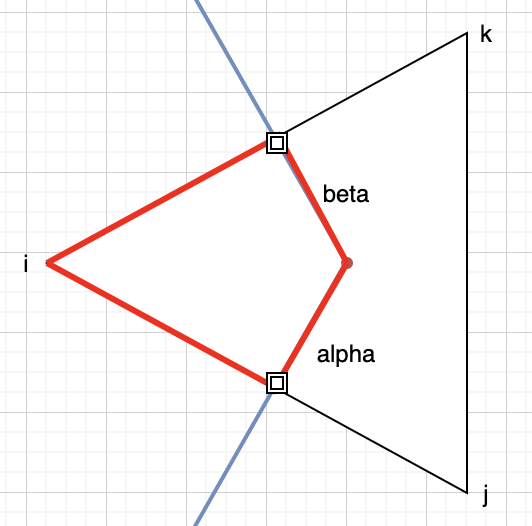
\includegraphics[width=0.4\linewidth]{Materials/rewrite}
	\caption{The cleverly constructed closed surface, where the edge pieces from vertex \textit{i} to vertex \textit{j} and \textit{k} are used along with the edge pieces $\alpha$ and $\beta$.}
	\label{rewrite}
\end{figure}
We can now rearrange the terms and get:
\begin{equation*}
	\int_{S^e_{\alpha}} \mathbf{P}^e\mathbf{N}dS + \int_{S^e_{\beta}} \mathbf{P}^e\mathbf{N}dS = -\int_{S^e_{ij}}\mathbf{P}^e\mathbf{N}dS - \int_{S^e_{ik}} \mathbf{P}^e\mathbf{N}dS
\end{equation*}
And we can now apply the midpoint approximation rule and define the internal forces:
\begin{align*}
	\mathbf{f}^e_i &=  -\int_{S^e_{ij}}\mathbf{P}^e\mathbf{N}dS - \int_{S^e_{ik}} \mathbf{P}^e\mathbf{N}dS\\
	&\iff -\frac{1}{2}\mathbf{P}^e\mathbf{N}^e_{ij}l^e_{ij} - \frac{1}{2}\mathbf{P}^e\mathbf{N}^e_{ik}l^e_{ik}
\end{align*}
Where the half comes from the fact we only need half of the edge lengths, and \textit{l} is the length of the edge. We now have:
\begin{equation*}
	m_i\ddot{\mathbf{x}}_i = \mathbf{f}^{ext}_i + \mathbf{f}^t_i + \sum_{e_{inner}} \mathbf{f}^{e_{inner}}_i
\end{equation*}
We can simplify this by defining $f^{total}_i =  \mathbf{f}^{ext}_i + \mathbf{f}^t_i + \sum_{e_{inner}} \mathbf{f}^{e_{inner}}_i$ and we then have:
\begin{equation*}
	m_i\ddot{\mathbf{x}}_i = \mathbf{f}^{total}_i
\end{equation*}

The last part is the time discretization. Here we want to discretize the velocity updates and positional updates. We know $\ddot{\mathbf{x}} = \dot{\mathbf{v}}$ and $\mathbf{v} = \dot{\mathbf{x}}$, thus we have:
\begin{align}
	\dot{\mathbf{v}}_i &= \frac{1}{m_i}\mathbf{f}^{total}_i \label{sub1}\\
	\dot{\mathbf{x}}_i &= \mathbf{v}_i\label{sub2}
\end{align}
We can now use a forward difference approximation to approximate $\dot{\mathbf{v}}_i$:
\begin{equation*}
	\dot{\mathbf{v}}_i \approx \frac{\mathbf{v}^{t+\Delta t}_i - \mathbf{v}^t_i}{\Delta t}
\end{equation*}
Substituting this in at \autoref{sub1}, we get:
\begin{equation*}
	\mathbf{v}^{t+\Delta t}_i = \mathbf{v}^t_i + \frac{\Delta t}{m_i}\mathbf{f}^{total}_i 
\end{equation*}
We now have an explicit velocity update as the total force is updated at time \textit{t}.\\
We can now use a forward difference approximation for the $\dot{\mathbf{x}}$:
\begin{equation*}
	\dot{\mathbf{x}}_i \approx \frac{\mathbf{x}^{t+\Delta t}_i - \mathbf{x}^t_i}{\Delta t}
\end{equation*}
Substituting this into \autoref{sub2} we get:
\begin{equation*}
	\mathbf{x}^{t+\Delta t}_i = \mathbf{x}^t_i + \Delta t \mathbf{v}^{t+\Delta t}_i 
\end{equation*}
Because we just updated the velocities this becomes an implicit positional update.\\

We can now set up a simulation loop consisting of 9 steps:
\begin{enumerate}
	\item Compute deformation gradient $\mathbf{F^e}$ for all \textit{e}.
	\item Compute Green strain tensor $\mathbf{E}^e$ for all \textit{e}.
	\item Compute second Piola-Kirchhoff stress tensor $\mathbf{S}^e$ for all \textit{e}.
	\item Compute first Piola-Kirchhoff stress tensor $\mathbf{P}^e$ for all \textit{e}.
	\item Compute elastic forces  $\sum_{e_{inner}} \mathbf{f}^{e_{inner}}_i$ for all \textit{i}.
	\item Compute total forces $\mathbf{f}^{total}_i$ for all \textit{i}.
	\item Compute velocity update $\mathbf{v}^{t+\Delta t}_i$ for all \textit{i}.
	\item Compute position updates $\mathbf{x}^{t+\Delta t}_i$ for all \textit{i}.
	\item Increment time $t = t + \Delta t$, and begin anew from step 1.
\end{enumerate}